%\documentclass[a4paper]{article}
%\usepackage[top=1in, bottom=1.25in, left=1.25in, right=1.25in]{geometry}
%\usepackage{amsmath}
%\usepackage{multicol}
%\usepackage{graphicx}
%\usepackage{subfig}
%\usepackage{amssymb}
%%\RequirePackage{ltxcmds}[2010/12/07]
%%opening
%\title{Linear Filtering in Frequency-Domain}
%\author{ }
%\date{ }
%\begin{document}
%
%\maketitle
%Python code highlighting
\definecolor{mygreen}{rgb}{0,0.6,0}
\definecolor{mygray}{rgb}{0.5,0.5,0.5}
\definecolor{mymauve}{rgb}{0.58,0,0.82}

\lstset{ %
	backgroundcolor=\color{white},   % choose the background color; you must add \usepackage{color} or \usepackage{xcolor}; should come as last argument
	basicstyle=\footnotesize,        % the size of the fonts that are used for the code
	breakatwhitespace=false,         % sets if automatic breaks should only happen at whitespace
	breaklines=true,                 % sets automatic line breaking
	captionpos=b,                    % sets the caption-position to bottom
	commentstyle=\color{mygreen},    % comment style
	deletekeywords={...},            % if you want to delete keywords from the given language
	escapeinside={\%*}{*)},          % if you want to add LaTeX within your code
	extendedchars=true,              % lets you use non-ASCII characters; for 8-bits encodings only, does not work with UTF-8
	frame=single,	                 % adds a frame around the code
	keepspaces=true,                 % keeps spaces in text, useful for keeping indentation of code (possibly needs columns=flexible)
	keywordstyle=\color{blue},       % keyword style
	stringstyle=\color{red},
	language=C++,                    % the language of the code
	morekeywords={*,...},            % if you want to add more keywords to the set
	numbers=left,                    % where to put the line-numbers; possible values are (none, left, right)
	numbersep=5pt,                   % how far the line-numbers are from the code
	numberstyle=\tiny\color{mygray}, % the style that is used for the line-numbers
	rulecolor=\color{black},         % if not set, the frame-color may be changed on line-breaks within not-black text (e.g. comments (green here))
	showspaces=false,                % show spaces everywhere adding particular underscores; it overrides 'showstringspaces'
	showstringspaces=false,          % underline spaces within strings only
	showtabs=false,                  % show tabs within strings adding particular underscores
	stepnumber=2,                    % the step between two line-numbers. If it's 1, each line will be numbered
	stringstyle=\color{mymauve},     % string literal style
	tabsize=2,	                   % sets default tabsize to 2 spaces
	title=\lstname                   % show the filename of files included with \lstinputlisting; also try caption instead of title
}
\clearpage
\section{Filter}
\begin{refsection}
\begin{tcolorbox}	
	\begin{tabular}{p{2.75cm} p{0.2cm} p{10.5cm}}
		\textbf{Header File}   &:& filter\_*.h \\
		\textbf{Source File}   &:& filter\_*.cpp \\
		\textbf{Version}       &:& 20180201 (Romil Patel)
	\end{tabular}
\end{tcolorbox}
In order to filter any signal, a new generalized version of the filter namely $filter\_*.h$ \& $filter\_*.cpp$ is programmed which facilitate to filtering in both time and frequency domain. Basically, $filter\_*.h$ file contains the declaration two distinct class namely \textbf{FIR\_Filter} and \textbf{FD\_Filter} which help to perform filtering in time-domain (using impulse response) and frequency-domain (using transfer function), respectively (see Figure \ref{FilterClass}). The $filter\_*.cpp$ file contains the definitions of all the functions declared in the  \textbf{FIR\_Filter} and \textbf{FD\_Filter}.\\
\begin{figure}[h]
	\centering
	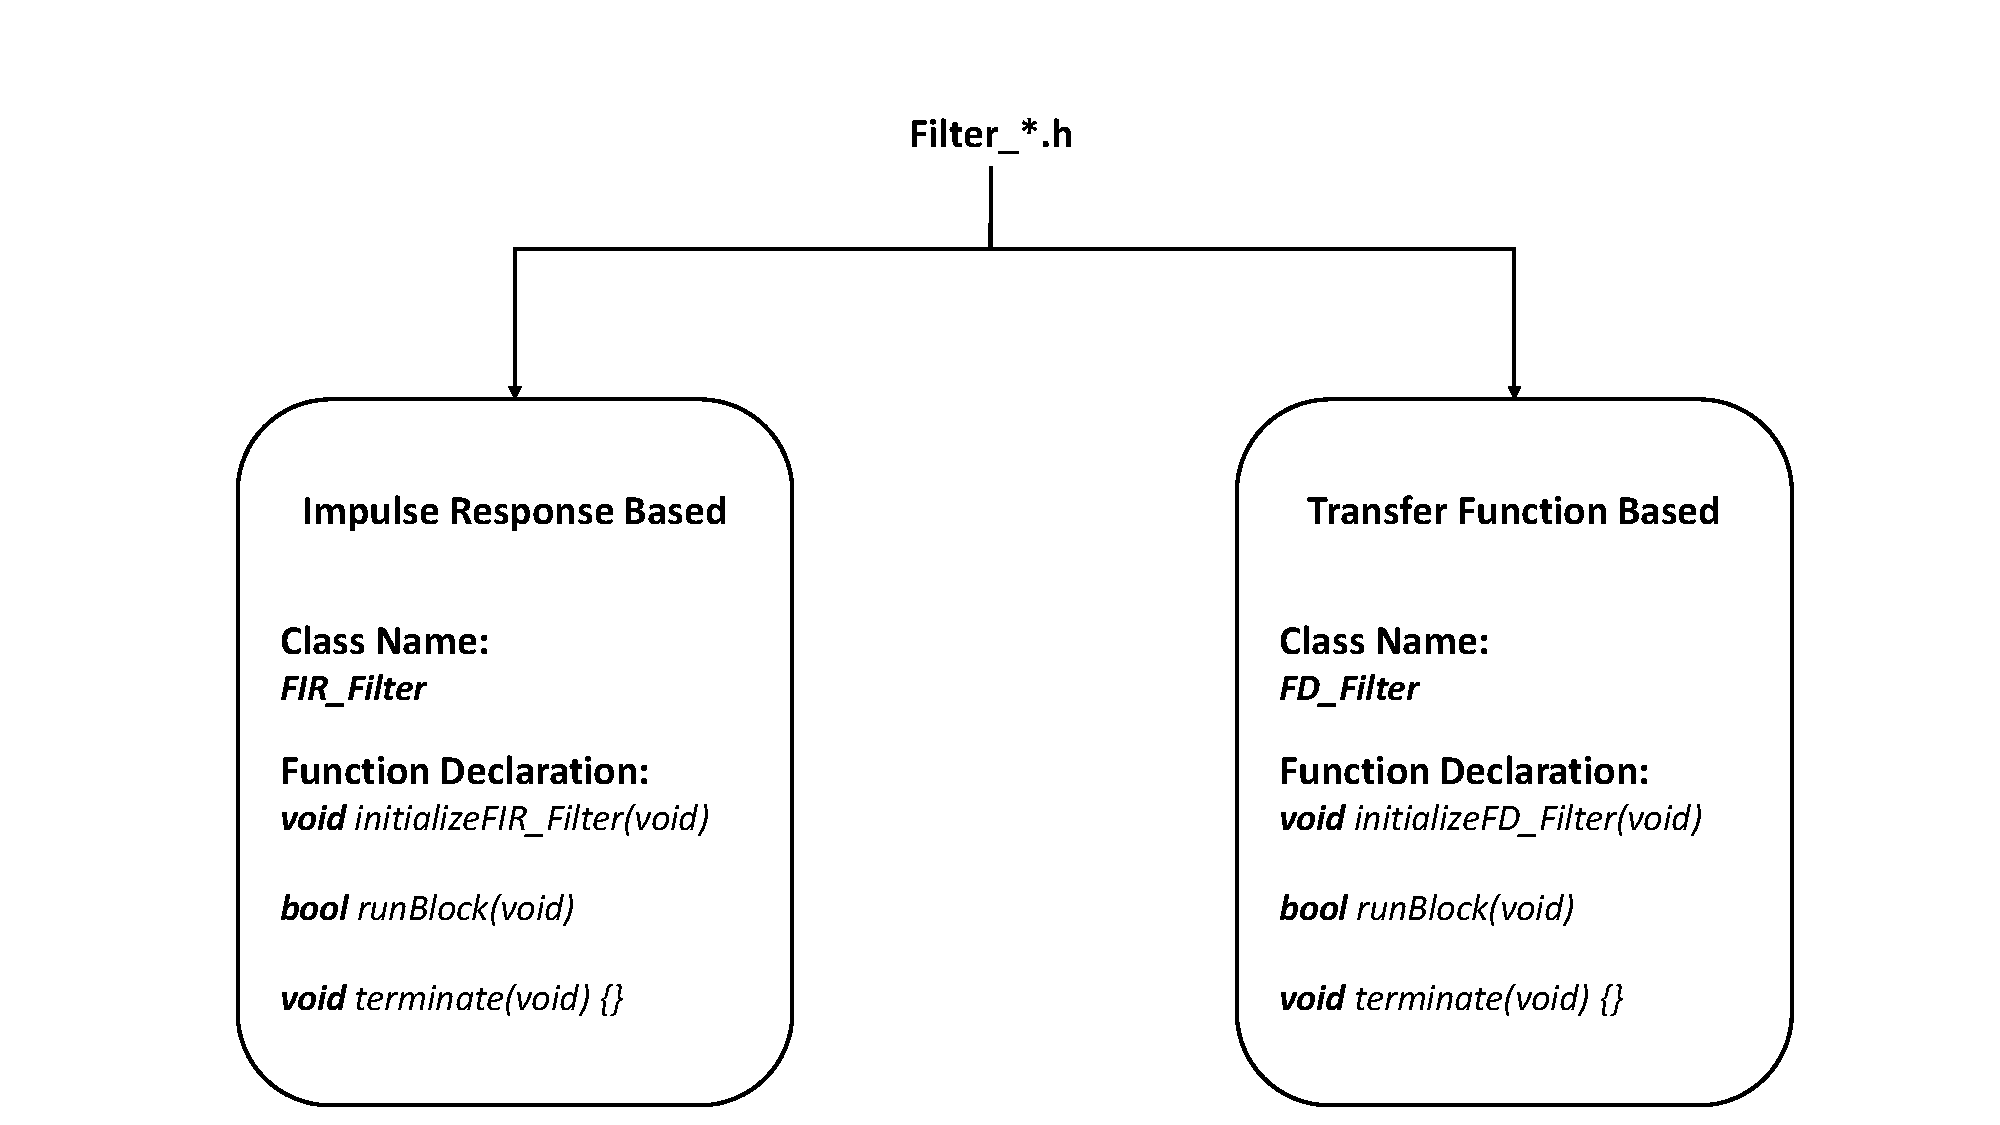
\includegraphics[width=16cm]{./algorithms/filter/figures/Filter_class.pdf}
	\caption{Filter class}
	\label{FilterClass}
\end{figure}
In the Figure \ref{FilterClass}, the function $\textbf{bool}$ $runblock(void)$ in the transfer function based \textbf{FD\_Filter} class, is the declaration of the real-time overlap-save method for filtering in the frequency domain. On the other hand, the function  $\textbf{bool}$ $runblock(void)$ in the \textbf{FIR\_Filter} class is the declaration of the function to facilitate filtering in the time domain \cite{Kuo,Rappaport2002} .\\
All those function declared in the $filter\_*.h$ file are defined in the $filter\_*.cpp$ file. The definition of $\textbf{bool}$ $runblock(void)$ function for both the classes are the following,
\lstinputlisting[firstline=34, lastline=58, language=C++, caption=Definition of \textbf{bool FIR\_Filter::runBlock(void)}]{../../algorithms/filter/filter_20180306.cpp}
\lstinputlisting[firstline=93, lastline=151, language=C++, caption=Definition of \textbf{bool FD\_Filter::runBlock(void)}]{../../algorithms/filter/filter_20180306.cpp}
Both the class of the filter discussed above are the root class for the filtering operation in time and frequency domain. To perform filtering operation, we have to include  $filter\_*.h$ and $filter\_*.cpp$ in the project. These filter root files require either \textit{impulse response} or \textit{transfer function} of the filter to perform filtering operation in time domain and frequency domain respectively. In the next section, we'll discuss an example of pulse shaping filtering using the proposed filter root class.

\subsection*{Example of pulse shaping filtering}
This section explains how to use \textbf{FIR\_Filter} and \textbf{FD\_Filter} class for the pulse shaping using the impulse response and the transfer function, respectively and it also compares the resultant output of both methods.
The impulse response for the \textbf{FIR\_Filter} class will be generated by a \textit{pulse\_shaper.cpp} file and the transfer function for the \textbf{FD\_Filter} will be generated by a \textit{pulse\_shaper\_fd\_20180306.cpp} file and applied to the $\textbf{bool}$ $runblock(void)$ block as shown in Figure \ref{Pulse_shaping}.
\begin{figure}[h]
	\centering
	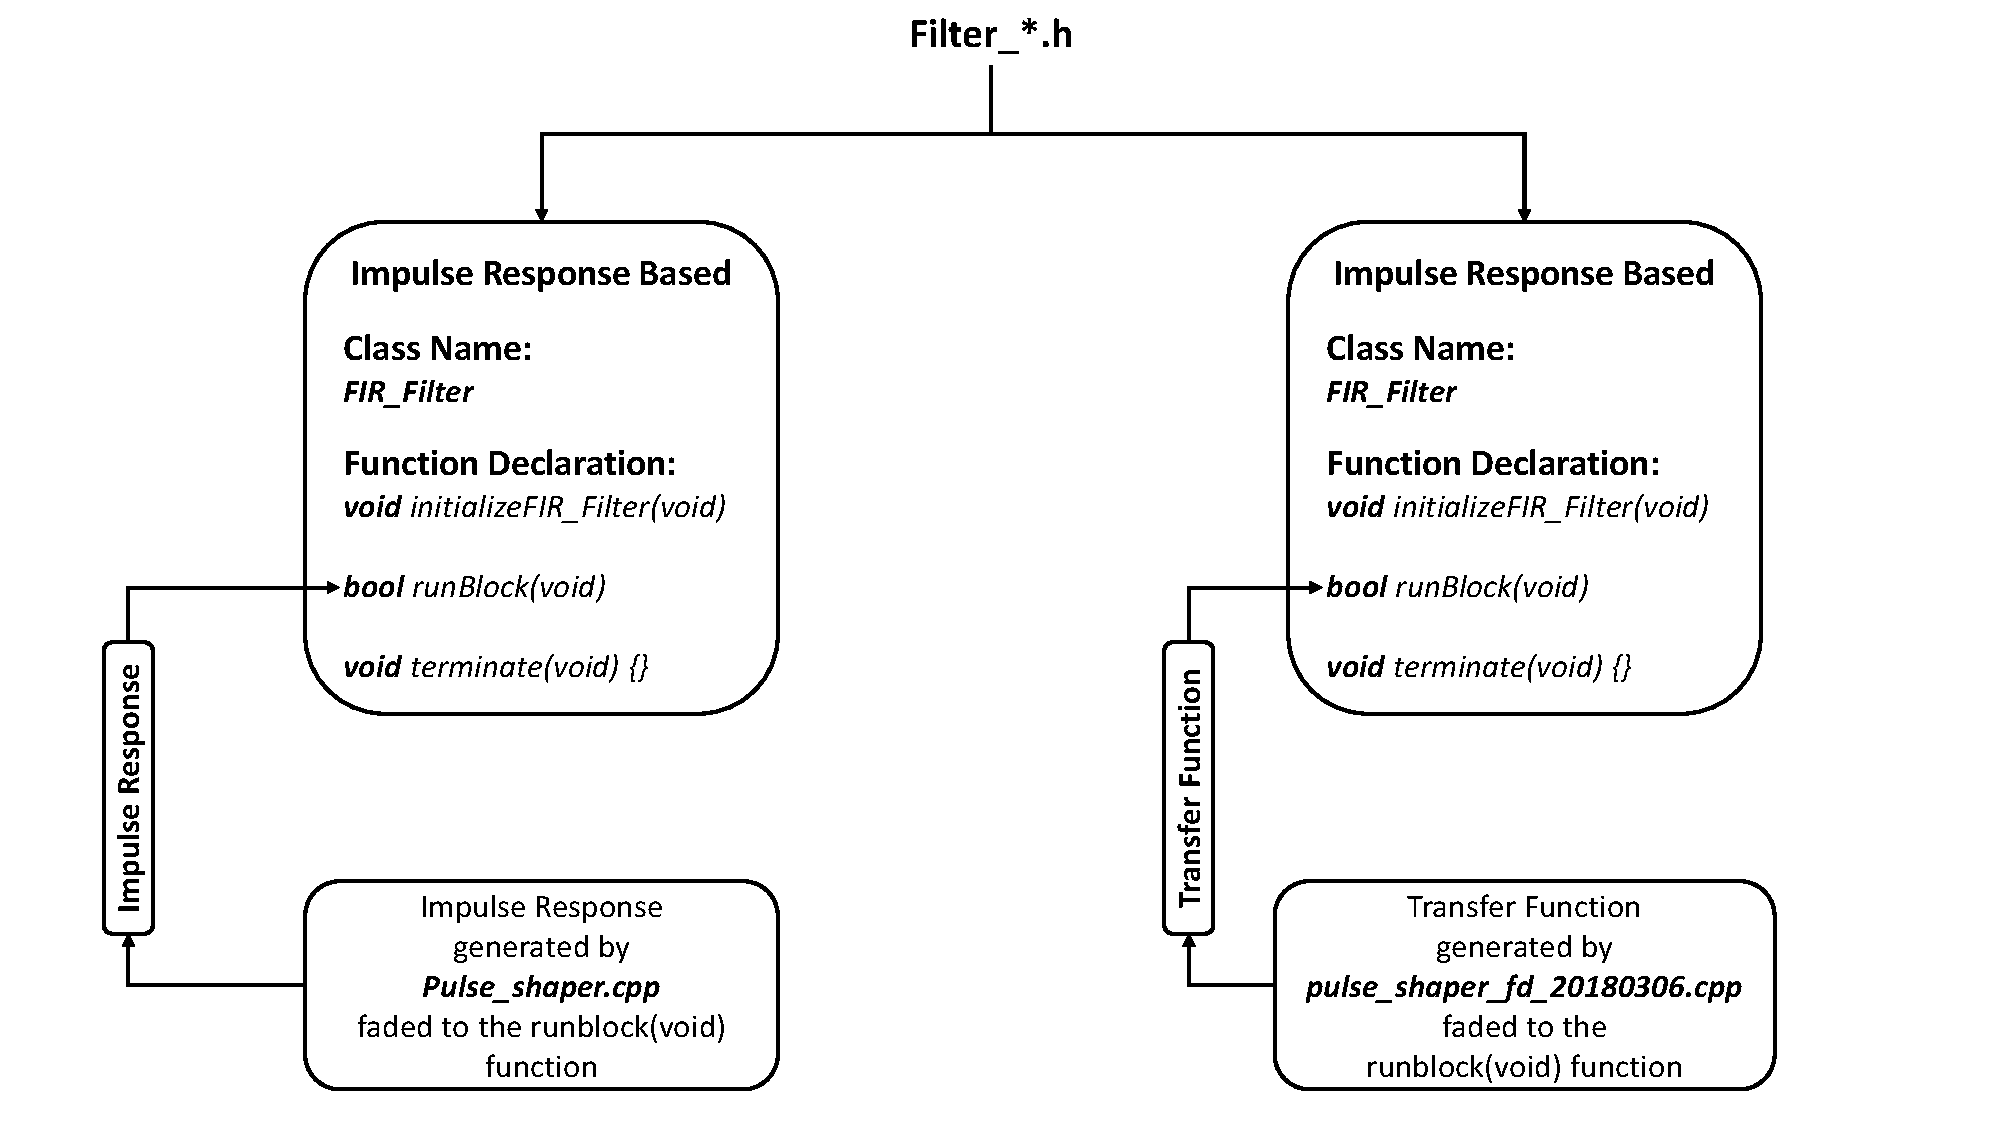
\includegraphics[width=17cm]{./algorithms/filter/figures/Pulse_shaping.pdf}
	\caption{Pulse shaping using \textbf{filter\_*.h}}
	\label{Pulse_shaping}
\end{figure}
\subsection*{Example of pulse shaping filtering : Procedural steps}
This section explains the steps of filtering a signal with the various pulse shaping filter using its impulse response and transfer function as well. It also displays the comparison between the resultant output generated by both the methods. In order to conduct the experiment, follow the steps given below:\\ \\
\textbf{Step 1} : In the directory, open the folder namely \textbf{filter\_test} by following the path  "/algorithms/filter/filter\_test".\\ \\
\textbf{Step 2} : Find the \textbf{filter\_test.vcxproj} file in the same folder and open it.\\
In this project file, find \textit{filter\_test.cpp} in $Source Files$ section and click on it. This file represents the simulation set-up as shown in Figure \ref{FilterTest}. \\ \\
\begin{figure}[h]
	\centering
	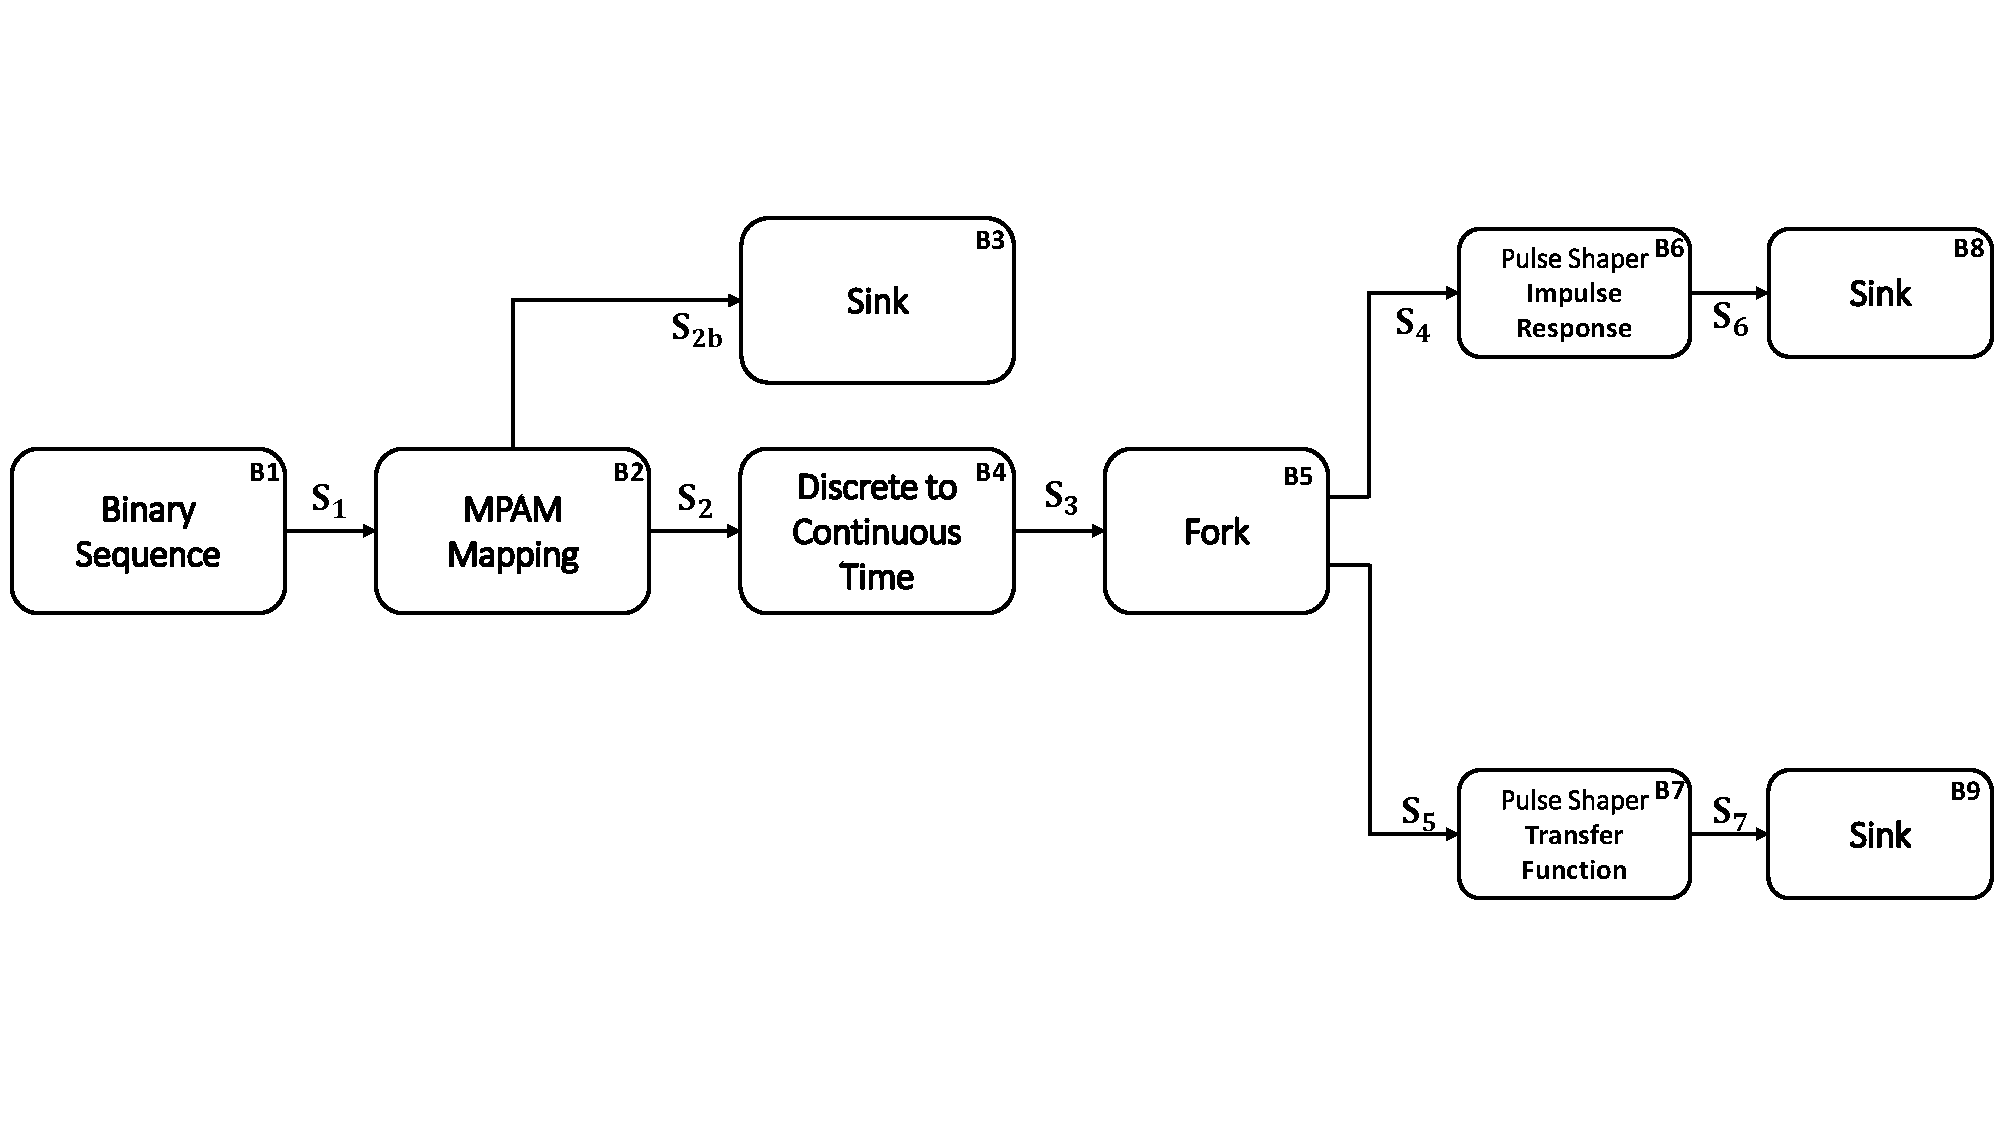
\includegraphics[width=16cm]{./algorithms/filter/figures/Test_Filter_Dia.pdf}
	\caption{Filter test setup}
	\label{FilterTest}
\end{figure}
\textbf{Step 3} : Check how \textbf{PulseShaper} and  \textbf{PulseShaperFd} blocks are implemented.\\
Check the appendix for the various types of pulse sapping techniques and what are the different parameters used to adjust the shape of the pulse shaper.\\ \\
%\lstinputlisting[firstline=73, lastline=84, language=C++, caption=Definition of \textbf{bool FIR\_Filter::runBlock(void)}]{../../algorithms/filter/filter_20180306.cpp}
\textbf{Step 4} : Run the \textit{filter\_test.cpp} code and compare the  signals \textbf{S6.sgn} and \textbf{S7.sgn} using visualizer.\\
Here, we have used three different types of pulse shaping filter namely, raised cosine, root raised cosine and Gaussian pulse shaper. The following Figure \ref{S6_S7}, \ref{S6_S7_RRCOS}  and \ref{S6_S7_gaussian} display the comparison of the output signals \textbf{S6.sgn} and \textbf{S7.sgn} for the raised cosine, root raised cosine and Gaussian pulse shaping filter, respectively. 

\subsection*{Case 1 : Raised cosine}
\begin{figure}[h]
	\centering
	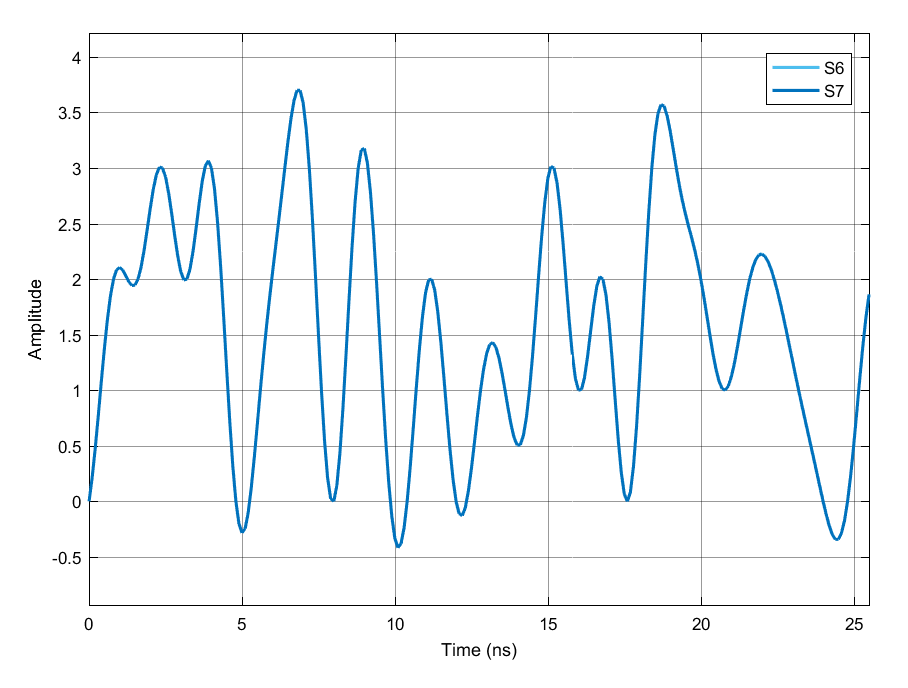
\includegraphics[width=10cm]{./algorithms/filter/figures/RC_S6S7.eps}
	\caption{Raised cosine pulse shaping results comparison}
	\label{S6_S7}
\end{figure}

\subsection*{Case 2 : Root raised cosine}
\begin{figure}[h]
	\centering
	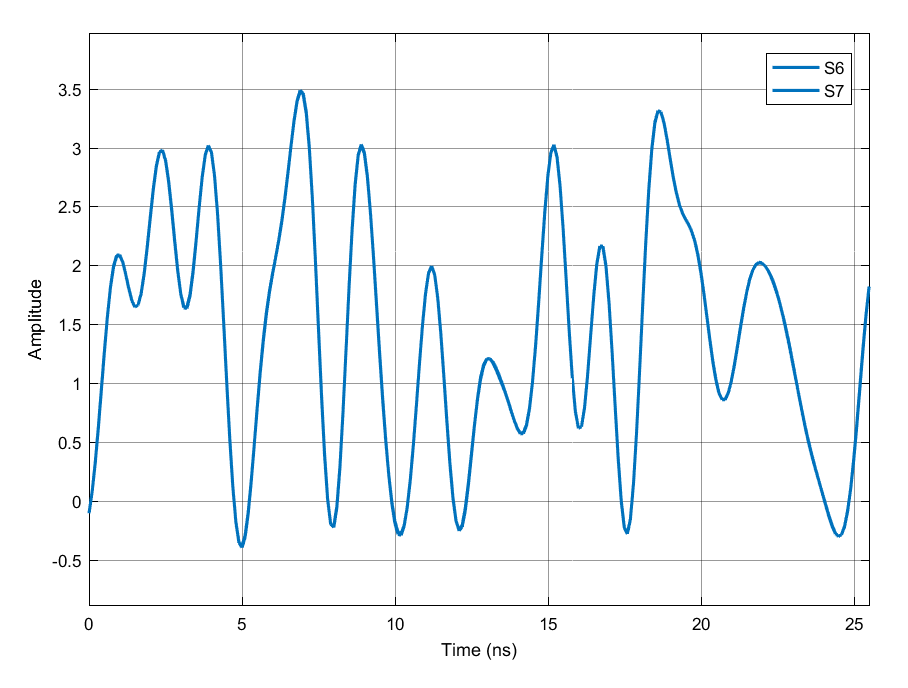
\includegraphics[width=10cm]{./algorithms/filter/figures/RRC_S6S7.eps}
	\caption{Root raised cosine pulse shaping result}
	\label{S6_S7_RRCOS}
\end{figure}

\subsection*{Case 3 : Gaussian}
\begin{figure}[h]
	\centering
	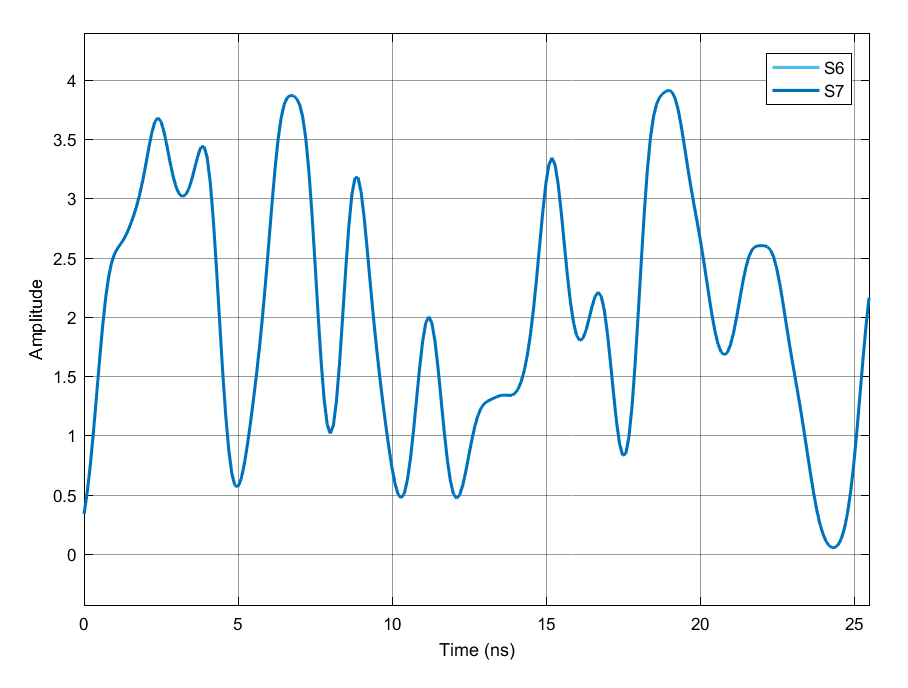
\includegraphics[width=10cm]{./algorithms/filter/figures/Gaussian_S6S7.eps}
	\caption{Gaussian pulse shaping results comparison}
	\label{S6_S7_gaussian}
\end{figure}



\section*{APPENDICES}
\subsection*{A. Raised cosine pulse shaper}
The raised cosine pulse shaping filter has a transfer function given by,
\begin{equation}
H_{RC}(f) = \begin{cases}
1 &\text{for $|f|\leq \dfrac{1-\beta}{2T_s}$}\\ \\
\dfrac{1}{2} \bigg[1 + cos\bigg(\dfrac{\pi Ts}{\beta}\bigg[|f|- \dfrac{1-\beta}{2T_s} \bigg]\bigg)\bigg] &\text{for $\dfrac{1-\beta}{2T_s}<|f|\leq\dfrac{1+\beta}{2T_s}$}\\ \\
0 & \text{otherwise}
\end{cases}
\end{equation}
The parameter, $\beta$ is the roll-off factor of the raised cosine filter. The impulse response of the raised cosine filter is given by,
\begin{equation}
h_{RC}(t) = \dfrac{sin(\pi t/T_s)}{\pi t/Ts}\dfrac{cos(\pi \beta t/Ts)}{1-4 \beta^2 t^2/T_{s}^2 }
\label{hRC}
\end{equation}
\subsection*{B. Root raised cosine pulse shaper}
The raised cosine pulse shaping filter has a transfer function given by,
\begin{equation}
H_{RC}(f) = \begin{cases}
1 &\text{for $|f|\leq \dfrac{1-\beta}{2T_s}$}\\ \\
  \sqrt{\dfrac{1}{2} \bigg[1 + cos\bigg(\dfrac{\pi Ts}{\beta}\bigg[|f|- \dfrac{1-\beta}{2T_s} \bigg]\bigg)\bigg]} &\text{for $\dfrac{1-\beta}{2T_s}<|f|\leq\dfrac{1+\beta}{2T_s}$}\\ \\
0 & \text{otherwise}
\end{cases}
\end{equation}
The parameter, $\beta$ is the roll-off factor of the raised cosine filter. The impulse response of the root raised cosine filter is given by,
\begin{equation}
h_{RRC}(t) = \begin{cases}
	\dfrac{1}{T_s}\bigg(1+\beta\big(\dfrac{4}{\pi}-1\big)\bigg) &\text{for $t = 0$}\\ \\
	\dfrac{\beta}{T_s \sqrt{2}}\bigg[ \bigg(1+\dfrac{2}{\pi} \bigg) sin\bigg(\dfrac{\pi}{4 \beta}\bigg) + \bigg(1-\dfrac{2}{\pi} \bigg) cos\bigg(\dfrac{\pi}{4 \beta}\bigg)  \bigg]  	&\text{for $t=\dfrac{T_s}{4 \beta}$}\\ \\
	\dfrac{1}{Ts}\dfrac{sin \bigg[\pi\dfrac{t}{T_s}(1-\beta)\bigg] + 4\beta\dfrac{t}{Ts}cos \bigg[\pi\dfrac{t}{T_s}(1+\beta)\bigg] }{\pi\dfrac{t}{T_s}\bigg[1-\bigg(4\beta \dfrac{t}{T_s}\bigg)^2\bigg]} & \text{otherwise}
\end{cases}
\end{equation}

\subsection*{C. Gaussian pulse shaper}
The Gaussian pulse shaping filter has a transfer function given by,
\begin{equation}
H_G(f) =exp(-\alpha^2 f^2)
\label{GPS}
\end{equation} 
The parameter $\alpha$ is related to B, the 3-dB bandwidth of the Gaussian shaping filter is given by,
\begin{equation}
\alpha =\dfrac{\sqrt{ln2}}{\sqrt{2}B}=\dfrac{0.5887}{B}
\label{Bandwidth}
\end{equation} 
From the equation \ref{Bandwidth}, as $\alpha$ increases, the spectral occupancy of the Gaussian filter decreases. The impulse response of the Gaussian filter can be given by,
\begin{equation}
h_G(t) =\dfrac{\sqrt{\pi}}{\alpha} exp(-\dfrac{\pi^2}{\alpha^2} t^2)
\label{IR}
\end{equation} 
From the equation \ref{Bandwidth},  we can also write that,
\begin{equation}
\alpha =\dfrac{0.5887}{BT_s}T_s
\label{Bandwidth2}
\end{equation} 
Where, $BT_s$ is the 3-dB bandwidth-symbol time product which ranges from $0\leq BT_s \leq 1$ given as the input parameter for designing the Gaussian pulse shaping filter.




% bibliographic references for the section ----------------------------
\clearpage
\printbibliography[heading=subbibliography]
\end{refsection}
\addcontentsline{toc}{subsection}{Bibliography}
\cleardoublepage
% --------------------------------------------------------------------- 



